% CREATED BY DAVID FRISK, 2016

\chapter{Diskussion}

\begin{binge}
De tre nedanstående ska vara nånstans i diskussion.

De domänspecifika språken modellerar områden snarare än att vara problemlösare. \textit{Analys} exemplifierar detta väl. Det språket består av ett syntaxträd över algebraiska uttryck samt operationer som derivering och integration. Med hjälp av det kan man modellera uttryck och analytiska operationer på dem. Däremot löser det inte problem åt en. Man kan med andra ord inte mata in en differentialekvation och automatiskt få en lösning.

Hur bra våra moduler blev samt varför de inte är problemlösare utan modellerare istället.

När områden kodades upp till domänspecifika språk var det långt ifrån alla gånger
det kunde göras på en meningsfullt sätt \todo{Expandera, Vad betyder meningsfullt?}. 

\section{Blev vi nöjda med läromaterialet?}

blablabla

\section{Tillvägagångssättet av skapandet}

Tanke: I metod/teori varför vi valde att just Haskell o.s.v. Beskrivning av
vårt iterativa arbetssätt, hur vi sökte i mörkret. Här i diskussion kanske mer
varför det var nödvändigt...

Annan tanke: antingen separat resultat-kapitel för "misslyckade" försök, som
DSL för lutande plan, eller att vi har det här..

Vi har kanske inte varit så strukturerade, utan bara valt ut något område på
måfå som vi kände för, t.ex. valet av termodynmik.

Blev så för svårt att veta vad som DSL lämpligt för.

Största svårigheten var att välja områden som skulla passa bra för DSL. Som att
famla i mörkret.

Kan skriva om misslyckade försök att skapa DSLer för vissa saker. T.ex. lutande plan (DSL för det, ej problemlösning av det området med andra DSL:er), bevis med Haskells typsystem...

\section{Domänspecifika språk och fysik}

Hur en kombination av domänspecifika språk och fysik ser ut är inget uppenbart. Går det att kombinera de två, och för vilka områden fungerar det bra för? Slutligen, är det lärorikt att presentera fysik ur ett domänspecifikt-språk-perspektiv?

\subsection{Om läromaterialets fokus på matematik och Haskell snarare än fysik}

En stor del av läromaterialets fokus ligger på matematik och Haskell snarare än
fysik. Detta trots att läromaterialet är tänkt att handla om fysik. Varför är
det så?

En orsak till att ett stort fokus ligger på matematik är att fysik egentligen
bara är räkneexempel i matematik. Ta cirkulär centralrörelse som exempel. Att
beskriva en sådan rörelse hos en kropp görs med hjälp av vektorer och
matematisk analys. Fysik finns bara som en bakomliggande teori som dikterar
vilka samband som gäller. Själva räknandet görs sedan med matematik.

Detta är inte hela sanningen. Inom fysik ingår en stor del problemlösning, till
exempel att sätta upp och hitta krafter i mekanikproblem, utan att någon
matematik behöver blandas in. Denna typ av fysik är dock svår att göra
domänspecifika språk av, något som diskuteras djupare i avsnitt
\ref{sec:lampligt}.

Läromaterialet innehåller även en hel del förklaringar av Haskell-teknisk
karaktär. Orsaken till detta är tvåfaldigt. För det första
används avancerade koncept inom Haskell som läsaren inte förväntas kunna sedan
innan. Ett exempel är typnivå-programmering. För att göra kopplingen mellan
Haskell och fysik så tydlig som möjlig behövdes fysikaliska dimensioner kunna
likställas med, och hanteras på samma sätt, som Haskell-typer.

För det andra är läromaterialets syfte inte enbart att lära ut fysik i sig,
utan även visa hur fysik kan modelleras i domänspecifika språk och dra
paralleller mellan fysik och domänspecifika språk. Av detta skäl blir det
naturligt att det ''även'' ägnas en hel del förklaringar åt programkoden.
Syftet är att väcka intresse för fysik, inte att lära ut fysik. Ett sätt att
göra det är då att visa dessa paralleller.

Är det rätt eller fel att ha en relativt liten tyngd på fysiken som projekets
läromaterial har? På den frågan har vi mer än ett svar. Man kan svara ja, med
hänvisning till de ovanstående skälen att det direkta syftet inte är att lära
ut fysik utan att väcka intresse. Man kan svara nej, och hävda att de
domänspecifika språken kan utformas på ett annat sätt som mer direkt
knyter an till fysikaliska koncept, till exempel ett syntaxträd för
sammansättningen av ett lutande plans komponenter. Vi tyckte dock det var svårt
att göra på det sättet, se avsnitt \ref{sec:lampligt}. Detta är dock en
vidareutvecklingspotential, att undersöka huruvida det går att göra på ett bra
sätt.

Man kan svara nej på frågan av ett annat skäl också, nämligen att fysiken i sig
bör vara det främsta fokuset. Detta skulle dock innebära en helt annan form på
läromaterialet. Vi menar att det skulle vara svårt att väva in domänspecifika
språk på ett meningsfullt sätt om de samtidigt skulle vara i skymundan. Ett
läromaterial med större fokus på fysik bör i så fall enbart handla om fysik. En
utförligare diskussion om detta finns i avsnitt \ref{sec:bara_fysik}.

\subsection{Vad för slags områden är DSLs lämpligt att göra för?}
\label{sec:lampligt}

Under projektets gång gjordes flera experiment för att se hur man kunde göra ett domänspecifikt språk för ett område. Det visade sig att visa områden var lämpligare än andra. Till exempel var analys och vektorer områden som vi ansåg väl lämpade, medan andra som till exempel lutande plan och termodynamik var mindre lämpade.

Vad har de lämpliga områdena gemensamt? De gemensamma dragen är att de är matematiska, har en fix struktur och består av ''data och operationer''. Tabell \ref{tab:data_och_ops} visar några exempel på områden med sina data och operationer.

\begin{table}[tph]
\centering
\caption{Exempel på data och operationer i några domänspecifika språk.}
\label{tab:data_och_ops}
\begin{tabular}{@{}l|l@{}}
\toprule
DSL / data & Exempel på operationer \\ \midrule
Dimensioner & Multiplikation, division \\
Vektorer & Addition, skalärprodukt \\
Analys, funktioner & Derivera, multiplicera \\ \bottomrule
\end{tabular}
\end{table}

Varför gör dessa drag att de är lämpliga att göra domänspecifika språk för? TODO: Matematiska: man modellerar syntaxen

Den fixa strukturen kombinerat med data och operationer gör det enkelt att modellera med datatyper i Haskell. Datatyper har nämligen också en fix form. Dessutom blir relationen mellan å ena sidan data i fysik och datatyper i Haskell, å andra sidan operationer i fysik och funktioner i Haskell, väldigt tydlig. En operation/funktion resulterar sedan i data av samma slag som innan.

Denna strukturella likhet gör modellerandet och manipulerandet av data enkel att genomföra rent tekniskt. Men den innebär också en pedagogisk vinst. Genom att ha strukturerat upp fysik tydligt i Haskell blir det förhoppningsvis enklare för läsaren att förstå hur datan hänger ihop rent fysikaliskt.

I kontrast till dessa lämpliga områden står mindre lämpliga områden (eller åtminstone som vi inte lyckades göra något bra till). Som nämndes tidigare är termodynamik och lutande plan exempel på mindre lämpliga områden. Vad har dessa områden för gemensamma drag?

Ett gemensamt drag som gör dem svåra att göra domänspecifika språk av är att de består av en samling teoretiska samband. För det lutande planet är det till exempel $a = g * sin(v)$, som illusteras i figur \ref{fig:lutande_plan}.

\begin{figure}[tph]
  \frame{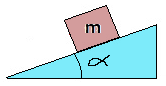
\includegraphics[width=\linewidth]{figure/lutande_plan.pdf}}
  \caption{Den variant av lutande plan som referas till i exemplet i texten. $a$ är en lådas acceleration längs med planet, $g$ är tyngdacceleration och $v$ är vinkeln. Friktionen antas vara försumbar.}
  \label{fig:lutande_plan}
\end{figure}

Teoretiska samband av det slaget relaterar olika egenskaper i systemet. Visserligen kan man modellera samband och ekvationer som ett domänspecifikt språk, men vi menar att nyttan inte blir stor med det. Det man kan göra är att programmera en ekvationslösare. Men den hade behövt vara både mekanisk och komplex. Den skulle alltså skilja sig drastiskt från hur man löser problem för hand och skulle vara svår att förstå. Alldeles för mycket fokus skulle hamna på algoritmer istället för fysik.

När det kommer till lutande plan och liknande områden är nyckeln att visserligen känna till vilka samband som gäller, men det framförallt att veta när man ska använda dem och hur man tillämpar dem på olika typer av uppgifter. Vi behandlar därför områden som lutande plan genom att lösa exempeluppgifter modellerade i de tidigare domänspecika språk. De tidigare språken tillhandahåller de matematiska verktyg som behövs för att koda upp lösningar av problem.


TODO: Kanske avsluta med att poängtera skillnaderna mellan lämpliga och mindre lämpliga.

Och vad är skillnaden mellan dessa två kategorier av områden?

Den viktiga skillnaden är att t.ex. analys har tydlig data och operationer
medan problemlösning som lutande plan har ett gäng samband som man använder
beroende på behov.

\subsection{Gör DSLs så att fysik blir mer lättförståeligt eller intressant?}
\label{sec:bara_fysik}

Är det pedagogiskt att lära ut fysik genom att presentera den med hjälp av domänspecifika språk? Väcker det intresse för fysik?

Ex med värde-nivå dims. Skoj att se hur ett objekt av nåt slag kan kodas upp. Blir mer strukturerat då.

Ex med lutande plan: man kan betrakta ett sådant problem som en samling ekvationer. Man har några kända värden och med hjälp av ekvationerna ska man hitta den sökta obekanta. Hjälper verkligen ett DSL till att man blir bättre på detta?

Med enheter, räcker det inte att förklara skillnaden mellan storheter, dimensioner och enheter på ett så grundligt sätt vi gjorde, utan att blanda in DSLs? Problemet i fysik för Data kanske är att det inte förklras grundligt och mycket är underförsått. Behöver man ens förstå enheter grundligare för att klara fysik bättre?

Man kan också se det som att DSLs och denna extrakunskap vi presenterat är för att göra fysik intressant genom att visa på vad för kopplingar till programmering man kan göra, även om områdena vi behandlat inte är direkt de områden som man behöver förstå för att klara kursen. Projektet kan ses som ren kuriosa som kan vara intressant.

Testgruppens åsikter här

\section{Inte tänkt så mycket på didaktik}

Fanns mycket i ARCS vi inte använder. Kanske därför inte kan förvänta oss att så bra pedagogiskt.

Men projekets fokus var snarare av teknisk karaktär.

Egentligen har det väl varit skapandet som varit det lärorika och inte användingen av det vi gjort?

\section{Vidareutvecklingsmöjligheter}

Läromaterialet innehåller domänspecifika språk för de \textit{matematiska} områdena analys och vektorer. Dessa områden används sedan för att koda upp och lösa uppgifter av mer \textit{fysikaliska} slag, till exempel lutande plan. Med andra ord görs inga domänspecifika språk för fysik i sig. En vidareutveckling hade därmed varit att göra precis det, att inte bara tillämpa matematiska domänspecifika språk utan göra fysikalsika domänspecifika språk. Det kan vara saker som ett syntaxträd för ett lutande plans komponenter. Det kan vara ett syntaxträd för vilka krafter som verkar på fysikalsika kroppar i mekanikproblem. Det kan till och med vara ett domänspecifikt språk för något så abstrakt som fysikalisk problemlösning i allmänhet. Vi har dessvärre ingen aning hur det skulle kunna se ut. Men av just detta skäl tror vi det hade varit väldigt intressant att se hur ett mer fysik-orienterat domänspecifikt språk kan se ut.

En annan möjlig vidareutveckling är att göra en rigorös studie kring de pedagogiska aspekterna kring kombinationen av fysik och domänspecifika språk. Detta projekt innehöll enbart en mindre sådan studie. Det som kan vara intressant att undersöka är om studenter tycker att fysik blir intressantare genom en kombination av detta slag och kanske därför studerar mer i fysikkursen. Eller kanske om de rent av blir bättre på fysik i sig genom att fysik presenterats på detta sätt, det vill säga att ett läromaterial av detta slag skulle kunna fungera istället för traditionell undervisning inom fysik. Givetvis skulle kompletering av läromaterialet behöva göras så att det är heltäckande.

Slutligen kan det befintliga läromaterialet byggas vidare på. I sin nuvarande form behandlas varken termodynamik eller vågrörelselära något alls. Dessutom lär det finnas aspekter inom den klassiska mekaniken som fattas.

\section{Etiska aspekter}

En bakomliggande tanke vi haft genom hela projektet är att läromaterialet ska vara tillgängligt för alla. Därav har vi valt att publicera det på en hemsida. Denna hemsida använder grundläggande HTML och CSS samt javascript. Javasript är dock inget krav för funktionalitet. Eftersom hemsidan är lättviktig bör den fungera väl även på gamla datorer och telefoner, till skillnad från tunga PDF-filer och många moderna hemsidor.

Tanken om tillgänglighet ligger även bakom valet att låta källkoden var fritt tillgänglig. Visserligen \textit{är} läromaterialet i princip hela källkoden, så har man läromaterialet har man källkoden. Att ha källkoden dirket har dock fördelar som att man kan följa med i versionshistoriken, man kan se kommentarer och alternativa implementationer som inte syns i den slutgiltiga produkten samt att det blir enklare att modifera källkoden och man inte behöver reverse-enginnera hemsidan. Det handlar om att visa att man är positiv till att andra tittar hur man gjort och låta andra bygga vidare på ens skapelser. Genom att sluta oss till skaran som tillämpar öppen källkod hoppas vi att fler inom samhället i stort ska gå över till denna modell.

Valet att skriva på engelska har också att göra med tillgängligheten. Fler kan engelska än svenska. Så på detta sätt kan läromaterialet komma fler till gagn.

Roligt <-- vet ej hur ska få in bra.



Om Hemsidan: 
  Det är lite intressant ur pedagogik-aspekten. Kan det
  kanske vara lättare/roligare att lära sig om sidan är fin och
  lättläst? Att javascript inte krävs gör att sidan kan visas ordentligt
  även om man sitter i U-land med dålig/gammal/billig telefon.


\end{binge}
